
\section{Literature Review}
\subsection{Sentiment Analysis Tools}

Many existing sentiment analysis tools are tailored towards market research for businesses, so focus on providing opinion mining tools for social media. This means that they focus on extracting how positive or negative the text is (also referred to as the Valence), and the subject that is being discussed. In terms of obtaining an emotion from a piece of text, this binary structure of representing all possible sentiments is very limiting. Emotion can be argued as more than just a binary structure, either "Happy" or "Sad", so there is a considerable interest in exploring this further.

There seems to be very little existing work which tries to use semantic analysis to predict more than just the Valence of text, so comparing this to existing work is a challenge. Commercial solutions tend to present their final sentiment analysis models as an API for which can be harnessed for general use, and for further projects and an example of this is Amazon Comphrehend.

The Amazon Web Services (AWS) Platform offers Amazon Comprehend \cite{aws} as a sentiment analysis product to customers. This is a NLP tool that extracts attributes such as a positive or negative Valence, and entities such as locations that are being discussed in an input text. When tested with a misleading piece text, it does not predict the sentiment well, as shown in Figure \ref{aws:sentiment}. This sentence contains both positive and negative emotions within it, which is where the binary structure of representing emotion in one dimension is limiting. This is an example of where using a more complex structure to represent a sentiment can come into use. 

\begin{figure}[ht]
\centering
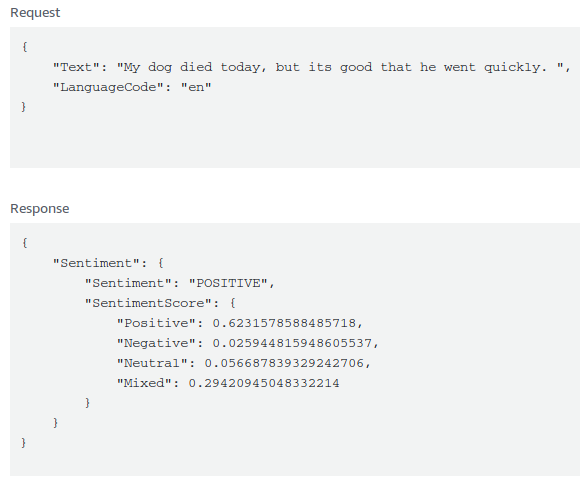
\includegraphics[scale=0.5]{litImgs/comphrendResult.png}
\caption{A display of the input text and incorrect analysis of the sentiment of it by the Amazon Comprehend service}
\label{aws:sentiment}
\end{figure}

\subsection{Sentiment Representation structures}

\subsubsection{Ekman's Six Basic Emotions}

There is no universally accepted model for representing sentiments, but a standard for classifying emotions in a categorical model is using Ekmans six basic emotions \cite{Ekman}. These are identified as Anger, Disgust, Fear, Happiness, Sadness and Surprise. Since there are only six discrete classes in which emotions can be placed, this can be argued to be very subjective when classifying \cite{emoBank}, but are very useful in portraying a general result back to user rather than numeric values.

\subsubsection{Valence}
A very common way to classify phrases and sentences in sentiment analysis is to analyse the Valence of the text, as already briefly discussed \cite{frijda1986emotions}.

The valence of a piece of text is how positive or negative is perceived to be, usually rated on a scale between 0 and 1, with 0 being very negative.
Using valence in a machine learning context is very useful, since many textual datasets exist that are already split into how positive a piece of text is, such as product or movie reviews which are frequently accompanied by a star rating. There is plenty of previous projects that use this as a way to represent emotion, taking in input text and outputting a Valence value usually on a numeric scale. so this is a good base to structure a more complex model on.

\subsubsection{Valence Arousal Dominance Structure}

The Valence-Arousal-Dominance (VAD) structure provides a 3D representation for emotions, with each variable being defined as follows \cite{VAD}:
\begin{itemize}
    \item Valence- How positive or negative the statement is.
    \item Arousal- Degree of calmness or excitement, the energy of the statement. 
    \item Dominance- Degree of control over a situation.
\end{itemize}

This structure provides the extra information about an emotion that is needed for a more in depth analysis of text, so will be used as the scale to analyse input text with for this project.

Using VAD values allows for easy representation into the Ekman six basic emotions as well,as there has been a standard for translating between them \cite{VADMapping}, shown in Table \ref{ekmansTable}.


\begin{table}[ht]
\caption{Ekmans emotions mapped to VAD values \cite{VADMapping}}
\centering
\begin{tabular}{ |c|c|c|c|c|c|c| } 
 \hline
  & Anger & Disgust & Fear & Happiness & Sadness & Surprise \\ 
 \hline                        
 Valence & 1.23 & 1 & 0.9 & 4.53 & 0.93 & 3.5\\ 
 Arousal & 3.98 & 3.38 & 4 & 3.78 & 1.83 & 4.18\\ 
 Dominance & 3.13 & 2.78 & 1.43 & 3.65 & 1.68 & 2.18\\ 
 \hline
\end{tabular}
\label{ekmansTable}
\end{table}


\subsection{Available Data}
There are two suitable datasets for this task, with data in two distinct styles which both use a VAD structure to rate input text on.

\subsubsection{Bag-of-Words}

The bag-of-words dataset contains 14,000 English words, each with a specific VAD value assigned \cite{wordsData}. Building a prediction model with this dataset would lose any context in which the words are in within a sentence, so is not ideal for this task, but using it to create a lexicon-based bag of words style prediction model will be investigated.

\begin{figure}[h]
\centering
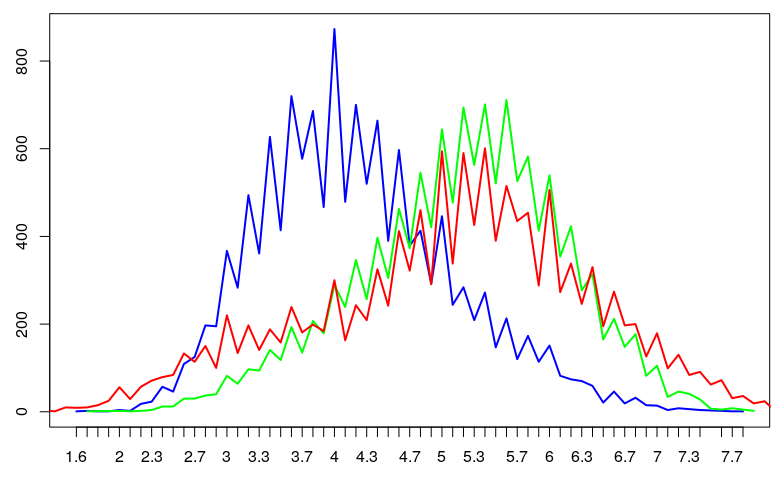
\includegraphics[scale=0.4]{graphs/lexiconDist.png}
\caption{Frequency of words over each dimension in bag-of-words dataset R: Valence, B: Arousal, G: Dominance. The dataset ranks the words on a scale between 0 and 10, which is adjusted for use with the EmoBank dataset}
\label{lexiconGraph}
\end{figure}

As we can see from Figure \ref{lexiconGraph} there is a bias in the data for each dimension, and the average value for the Arousal dimension is noticeably lower than the other two. Whether this affects the suitability of this dataset for use in building a prediction model will be explored further.

\subsubsection{EmoBank}
This dataset is the most important one for this project, as it contains 10,000 English sentences covering multiple genres, all annotated with their own VAD values \cite{emoBank}.

This dataset contains values for each sample sentence from both the writer and the reader of the text, but due to the findings in the paper accompanying it \cite{emoBank}, only the values given by the reader will be used, as it concluded that this perspective has higher emotionality and therefore they should be easier to build a more accurate model with.

Many existing sentiment analysis tools train over very large datasets, scraping information from things such as movie reviews \cite{socher2013recursive} or from Tweets \cite{towardsDS}, and so usually have above 100,000 samples to train from. In this case, the EmoBank dataset only contains 10,000 sentences, and whether this is a setback will be investigated. These larger datasets could not be used in this case since they are not annotated in a way that allows a more complex emotion to be calculated, since they are usually only scored by their Valence values. 

\todo{what is imbalanced data}

\begin{figure}[h]
\centering
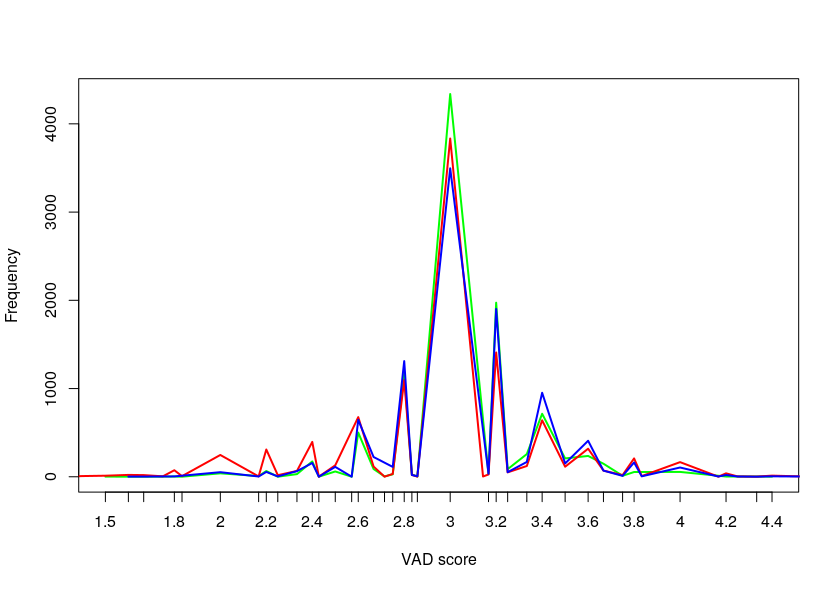
\includegraphics[scale=0.5]{graphs/VADdistribution.png}
\caption{Graph showing data distribution over the Emobank Dataset. R: Valence, B: Arousal, G: Dominance}
\label{dist:vad}
\end{figure}

\section{Problem Formulation}

Coming to a decision to use the VAD structure to analyse the sentiment of text and selecting two valid datasets to use means that the research questions set out can be broken down further.

\subsection{How can textual sentiment prediction be optimised?}

This can be refined into the following: 

\begin{enumerate}
    \item Ensuring the input text into the model is best suited to the type of analysis that will be carried out over it. 
    \item Analysing what the existing best text based sentiment prediction methods are and adapting them for predicting VAD values. 
    \item How to deal with a limited and imbalanced dataset, such as the Emobank dataset.
\end{enumerate}

To be able to answer these points in a formal way, we can set the base structure of the sentiment prediction model as shown in Figure \ref{intial:flow}. 
Text will be taken in in the form of sentences, and output values for the Valence, the Arousal and the Dominance of the text will be given from the model. The output format of the model for each of these dimensions will be based on how the dataset is processed by the model, which will be explored.

\begin{figure}[h]
\centering
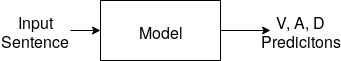
\includegraphics[scale=0.5]{litImgs/initialFlow.png}
\caption{Diagram showing the flow of data through the sentiment analysis model}
\label{intial:flow}
\end{figure}


\subsubsection{Data Pre-Processing Approaches}

To ensure the input text is in the best format for carrying out sentiment analysis upon, previous work has been analysed to ascertain which methods have been shown to lead to positive results.
R. Kim's series on investigating sentiment in twitter data \cite{towardsDS} has been very influential in this project for inspiring different ways that the data can be pre-processed so that any predictions can be optimised.
The two main ways that this experiment is done is by varying the N-Gram value and number of features supplied to the model.

To preserve the relationship between the words in the sentence, N-grams are very useful since it can help maintain negation of words and helps maintain the overall sentiment given in the sample sentence better. The number of features in this case is the most frequent N-Gram "words" that appear in the dataset.

\begin{figure}[h]
\centering
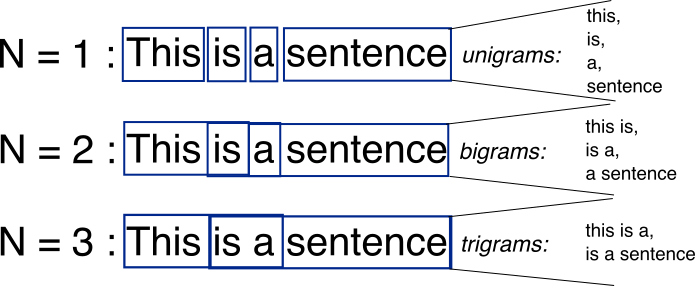
\includegraphics[scale=0.5]{litImgs/ngrams.png}
\caption{Diagram showing the way that the n-grams are created}
\end{figure}


During the experiments put forward by R. Kim, unigrams, bigrams and trigrams are compared and analysed over a feature range of 10000 to 100001. These experiments are done over a totally balanced dataset, with 50\% of the data being classed as having a positive valence, and the other 50\% with a negative one, and produce results as shown in Figure \ref{towards:DS} that imply that these methods are worth investigating, but can be improved upon.

\begin{figure}[h]
\centering
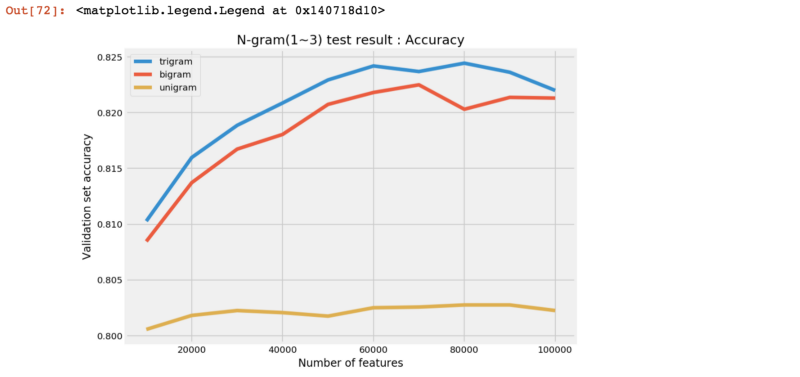
\includegraphics[scale=0.5]{litImgs/towardsDSNgramNFeatures.png}
\caption{Results from R. Kim's investigation for N-Gram and Number of Features selection for valence analysis over the Sentiment 140 Dataset \cite{go2016sentiment140}}
\label{towards:DS}
\end{figure}

Using these methods, our data flow through the system is now represented in Figure \ref{model:flow}.

\begin{figure}[h]
\centering
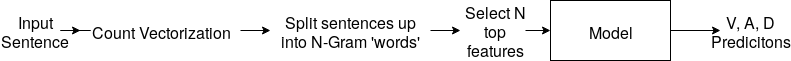
\includegraphics[scale=0.5]{litImgs/modelFlow.png}
\caption{Diagram showing inputs and outputs of the model}
\label{model:flow}
\end{figure}


\subsubsection{Model building approaches}

A common way of creating a semantic analysis tool is to use movie reviews, since these already have numeric values attached to them, or Twitter data due to the sheer volume of text available to create a prediction tool. Since previous sentiment analysis tools have all been done by training over datasets with the Valence values in discrete variables, Positive and Negative, sometimes with a Neutral class as well, the continuous variables given in the Emobank dataset will be bucketed into classes so that similar methods can be applied. An investigation into finding the optimal number of classes to split the data for each VAD dimension into will be carried out.
The output values for each dimension from the model will be the class, so 

When analysing the valence of tweets, using a lexicon based model, as well as implementing machine learning approaches have been used to great effect \cite{kolchyna2015twitter}, and hence these will be the methods investigated the creation of a prediction model.

There has been only a little research into using a multi-dimensional VAD structure to investigate sentiment, one paper primarily explores whether using a VAD structure could be used to help identify burnout in software developers \cite{mantyla2016mining}. In this case, a correlation was found between each of the VAD dimensions and issues raised in messages from the developers, meaning that there is an argument for using multiple dimensions to help understand textual data to a greater degree. An issue with this research is that they only used a word based lexicon where each individual word was assigned a value. This loses the context in which each word is being used in, and by using n-grams this issue will be mitigated.

Before exploring machine learning approaches, a lexicon based model will be established. This is using the bag-of-words dataset, \cite{wordsData} where each individual word in the input sentence is looked up in the dataset, assigned a value, then an average can be taken over the input sentence to give a resultant VAD score. This method has been used before to great effect with binary valence classification, and so investigating it in this case should lead to promising results \cite{kolchyna2015twitter}.

When choosing the machine learning based classifiers to investigate, literature shows that the same few classifiers tend to show the best results for analysing textual data.\cite{kolchyna2015twitter} \cite{frank2006naive}. \todo{which ones?}

Generally for semantic analysis machine learning models, Logistic Regression is popular, due to it being linear and scalable for large datasets \cite{towardsDS}. This is the model that will be initially used for comparing data pre-processing results.
Other classifiers that have been shown to give positive results for textual analysis tasks are different styles of Bayes classifiers,  which depend slightly on how many classes are being used. Multinomial is the most common for text categorisation problems, so this one will also be of high interest. \cite{frank2006naive}

Support Vector Machines have also been used in the past for text classification purposes with a positive results, so these will be incorporated as well \cite{joachims1998text}.

Previous work tends to avoid using computationally expensive approaches such as K-Nearest Neighbours and Random Forests due to the size of the datasets being used, but since the Emobank dataset is not that large, it is worth investigating those models as well.

\todo{Add a paragraph to summarise the problems of the existing work on sentiment analysis, and set out the direction of the investigation done in your work}

To compare these models further, we will also take a note of a rough estimate time it take for each classifier to run, to give us an idea of how much computation each takes.


\subsubsection{Over and Undersampling}

Due to the imbalance of data across the Emobank dataset as shown in Figure \ref{dist:vad}, trying to mitigate the effects of this is a challenge that has different ways of being tacked, and one common way of doing this is through oversampling the minority classes in the data, creating a more balanced dataset. \cite{towardsDS}

Since manually inputting more data would take more time than is sensible, the most common way to oversample the data that we are given, is through SMOTE (Synthetic Minority Oversampling Technique). This uses a K-Nearest neighbours approach to create synthetic data of the existing minority samples , and has been shown to have positive results with general machine learning tasks but has been known to be problematic with textual data, due to not actually creating synthetic samples which make logical sense. Investigating this method is worthwhile, although the expected results are fairly unknown as it depends heavily on the data in the minority classes. SMOTE tends to be simpler for continuous data \cite{chawla2002smote}, but we are turning the VAD values into discrete classes so this may lead to more difficulty in creating synthetic samples with accurate VAD scores. Since we will also be applying SMOTE to textual data however, where the synthetic text is likely to not make any sense, the issues caused by this should be minimal in comparison. 

There are other popular oversampling techniques that exist as well, for example just randomly re-sampling the minority class, as well as ADASYN (Adaptive Synthetic Sampling) which is a a form of a SMOTE oversampler which works better for classifiers without clear class boundaries, which will also be investigated.

Another, slightly different approach is to undersample the data, removing less important samples from the majority class so that the dataset is more balanced. This in itself can cause issues since you are reducing the amount of data that can be trained off, and literature shows that it tends to not have positive results for textual data, but since it can be used in circumstances when there is not enough data in the minority class to create decent synthetic samples in oversampling, it is worth exploring in this case \cite{more2016survey}. There are different methods of undersampling, from randomly removing items from the majority class, to using the three variations of the NearMiss undersampler, which uses different ways of implementing K-Nearest neighbours to select suitable samples to remove. 

The flow of the data can now be represented by Figure \ref{model:finalFlow}.

\begin{figure}[h]
\centering
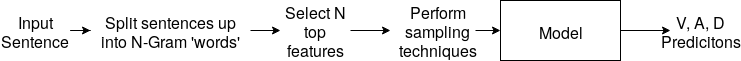
\includegraphics[scale=0.5]{litImgs/finalmodelflow.png}
\caption{Diagram showing the flow of data through the sentiment analysis model including over/undersampling techniques}
\label{model:finalFlow}
\end{figure}


\subsection{Does using more than 1 dimension to classify emotions provide more insight}

\subsubsection{Presenting Results}

Existing sentiment analysis tools either do not do anything with a final model, or use the tool as an API for use in general projects \cite{sentimentAPI}.  

To be able to present in the final model in a way that can be used to analyse whether we are able to establish more insight, an API will be created from it and web application that can access the data will be produced to allow for further analysis.

Music is also something  that cannot be easily classified into a binary sentimental structure, so relating the output VAD values of the produced model to songs is something that is worth exploring.

An existing product that does this is the MoodTape web application, which uses the valence of input text and relates this to the valence of a song  \cite{moodtape}. Since, as shown in Listing \ref{spotifyJSON}, much more information can be obtained from individual songs than just the valence, an improvement of this project would be to relate the Dominance and Arousal dimensions to some of the other attributes.

\begin{lstlisting}[style=leftCode, caption={Some of the attributes of a song obtained through requesting information through the Spotify API},captionpos=b, label={spotifyJSON}]
{
    "danceability": 0.322,
    "energy": 0.0593,
    "key": 1,
    "loudness": -53.057,
    "speechiness": 0.0444,
    "acousticness": 0.908,
    "instrumentalness": 0.708,
    "liveness": 0.121,
    "valence": 0.0165,
    "tempo": 158.402,
    "time_signature": 4
}
\end{lstlisting}

Using a web UI to present the results that has been done in the MoodTape application, and is probably the simplest way to gather all the data together, and so a simple web application will be produced. 

What we can class "more insight" as can be quite subjective, and as such discussions will be held with test users about how well they believe the predicted song fits them.